\documentclass[12pt,a4paper]{article}

\usepackage[french]{babel}
\usepackage[T1]{fontenc}
\usepackage[utf8]{inputenc}

\usepackage{amsmath,amsfonts,amssymb}

\usepackage{geometry}
\geometry{margin=75pt}

\usepackage[upright]{fourier}
\usepackage{subfig}

\usepackage{shadethm}

\usepackage{color}
\definecolor{gris_clair}{gray}{.9}
\definecolor{gris}{gray}{.35}
\definecolor{vert}{rgb}{0,0.5,0}
\definecolor{rouge}{rgb}{0.5,0,0}
\definecolor{turquoise}{rgb}{0,0.5,0.5}

\usepackage{listings}
\usepackage{paralist}
\usepackage{stmaryrd}
\usepackage{tikz}
\usetikzlibrary{shapes.multipart}
\usetikzlibrary{calc}


\title{Comment optimiser l'architecture d'un réseau pour résister aux attaques ?\\
Rapport final de TIPE}

\author{Dimitri Granger}


\begin{document}
\maketitle

\section{Préambule}
Mon objectif n'a pas changé depuis la MCOT. Mon but est donc resté la recherche de graphe robuste,
c'est à dire capables de rester connexe même après le retrait d'une partie de leurs arêtes ou noeuds. Dans ma 
modélisation il est également possible de protéger, avec un certain coût, des arêtes et des noeuds. Ma recherche a donc également portée sur la construction d'un graphe au coût minimal.

\section{Introduction}

Concevoir des réseaux capables de fonctionner après avoir été endommagés est crucial. J'ai donc étudié comment concevoir des réseaux capables de résister à des attaques d'ampleurs limitées.  J'ai modélisé ces réseaux avec des graphes non orientés. Les attaques sur un réseau sont modélisées par le retrait d'arêtes ou de nœuds du réseau. Les arêtes et noeuds des graphes pouvant être protégés avec un coût, j'ai recherché un graphe suffisamment robuste et de coût minimal en faisant varier les divers coûts, le nombre de noeuds du graphe et l'ampleur des attaques.



\section{Corps Principal}
\subsection{Modalités d'action}


J'ai représenté les graphes par des matrices d'adjacence. Pour limiter le temps de calcul de mes fonctions informatiques, j'ai tout d'abord fixé le nombre de nœuds $p$  à 15, et le nombre $k$ de nœuds ou d'arêtes qu'une attaque peut enlever à 10. Le but est alors de trouver comment relier ces 15 noeuds et comment répartir des protections pour créer un graphe robuste. La représentation des attaques se déroule de la manière suivante : on donne en entrée un graphe, et une liste aléatoire de nœuds et d'arêtes à attaquer est choisie. Parmi cette liste, les éléments non protégés sont supprimés du graphe. On utilise alors l'algorithme de Floyd-Warshall pour deux raisons : déterminer si le graphe résiduel est connexe, et pour calculer son diamètre. On calcule ensuite le coût $f$ du graphe avec la formule suivante :

\begin{math}


\begin{center}

                      f(c_{l},c_{d},c_{n}) = c_{n}p_{n} + c_{l}q + c_{d}q_{d}
											\smallbreak
\end{center}


\end{math}
\newline
avec $q$ le nombre d'arêtes, $c_{l}, c_{d},c_{n}$   le coût de formation d'une arête, de sa protection, et de la protection d'un noeud respectivement, $q_{d}$ le nombre d'arêtes protégées et $p_{n}$ le nombre de noeuds protégés.
Ce processus est renouvelé un grand nombre de fois, ici 1000, pour couvrir un grand nombre d'attaques possibles, et donc tester la robustesse du graphe considéré. 


\subsection{Restitution des résultats}
Deux graphes ressortent de cette expérience :
\begin{itemize}
\item Un graphe de Harary, c'est à dire avec $\lceil (p(k+1)/2) \rceil$ arêtes, ce qui est la taille minimale pour un graphe (k+1)-arêts connexe.
\item Un graphe en étoile, dont le nœud central et les arêtes sont protégés.
\end{itemize}

\begin{center}
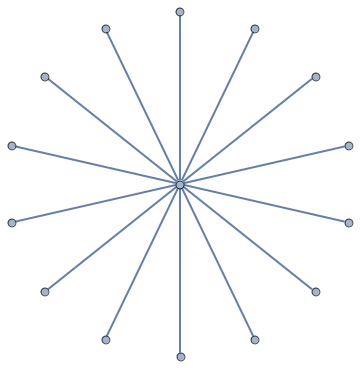
\includegraphics[width=0.49\linewidth]{C:/Users/Dimitri/Desktop/Stargraph.png}
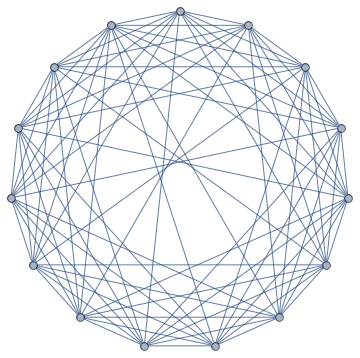
\includegraphics[width=0.49\linewidth]{C:/Users/Dimitri/Desktop/harary.png}
\captionof{figure}{Graphe en étoile et de Harary} 
\end{center}




J'ai donc étudié les fonctions de coût de ces graphes, en faisant varier le nombre de nœuds et le coût de chaque élément. Les fonctions de coût de ces graphes sont les suivantes :
\begin{itemize}
\item Graphe étoile : $f(c_{l},c_{d},c_{n}) = c_{n} + c_{l}(p-1) + c_{d}(p-1)$
\item Graphe de Harary : $g(c_{l}) = \lceil p(k+1)/2 \rceil c_{l}$
\end{itemize}

J'ai tout d'abord choisi de fixer $p$ à 15 nœuds, $k$ à 10, $c_{l}$ à 5, et de faire varier $c_{d}$ et $c_{n}$, et d'étudier $h = f-g$.
\begin{figure}[h]
	\centering
		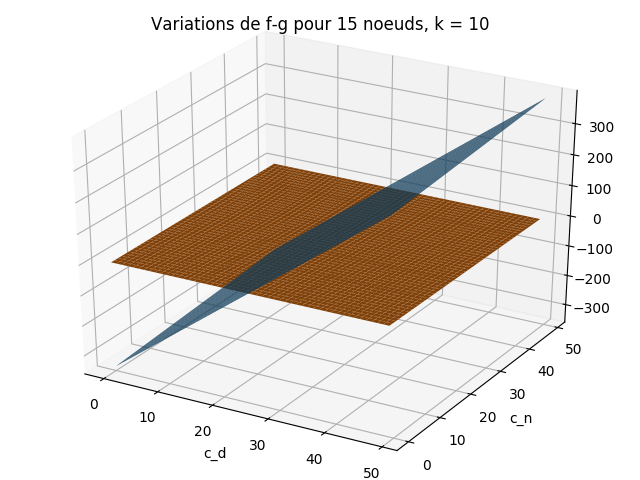
\includegraphics[width=0.49\linewidth]{C:/Users/Dimitri/Desktop/15noeuds10atk.png}
		\captionof{figure}{Variations de f-g pour p=15 et k=10.}
\end{figure}

On remarque que $c_{n}$ a peu d'influence, et que le graphe de Harary devient meilleur lorsque le coût de la protection d'une arête devient grand comparé à celui de la formation d'une arête.
J'ai choisi ensuite d'augmenter le nombre de nœuds à 500, puis de faire varier l'ampleur des attaques que peuvent subir les graphes.

\begin{center}
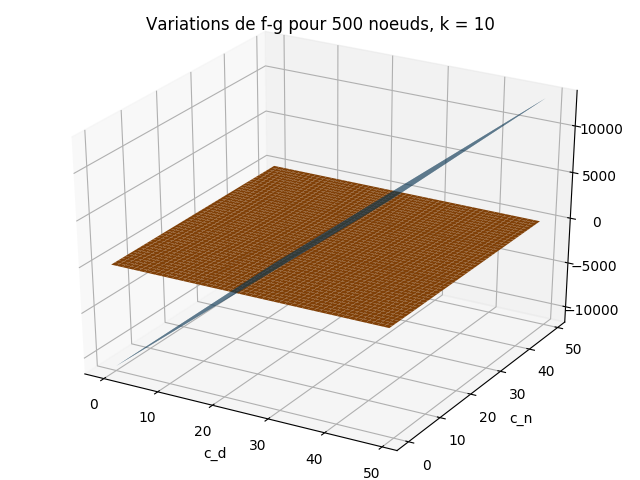
\includegraphics[width=0.49\linewidth]{C:/Users/Dimitri/Desktop/500noeuds10atk.png}
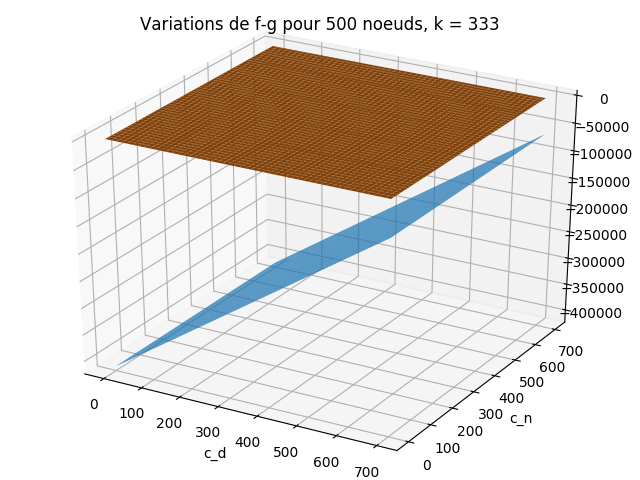
\includegraphics[width=0.49\linewidth]{C:/Users/Dimitri/Desktop/500noeuds333atk.png}
\captionof{figure}{Variations de f-g pour p=500, k=10 et k=333.} 
\end{center}

Si seul le nombre de nœuds varie, les résultats restent identiques. Cependant, si l'ampleur des attaques varie proportionnellement au nombre de nœuds, le coût d'un graphe de Harary devient largement supérieur à celui d'un graphe en étoile, à cause de la forte augmentation du nombre d'arêtes.

J'ai ensuite fixé $c_{d}$, $c_{n}$ et $c_{l}$ et étudié la variation des coûts de chaque graphe en fonction du nombre de nœuds dans le graphe.

\begin{center}
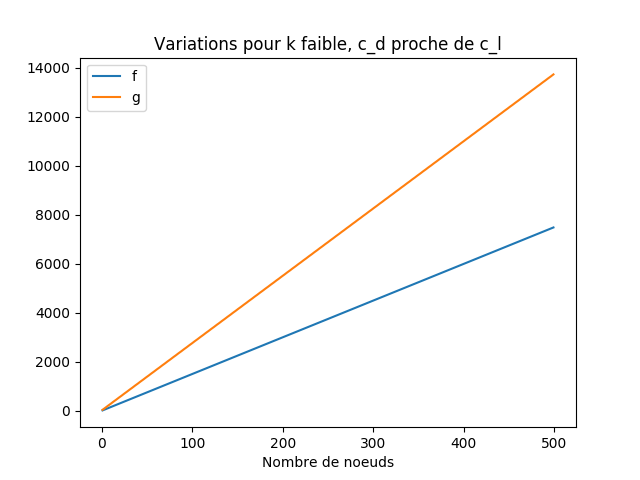
\includegraphics[width=0.49\linewidth]{C:/Users/Dimitri/Desktop/comp6.png}
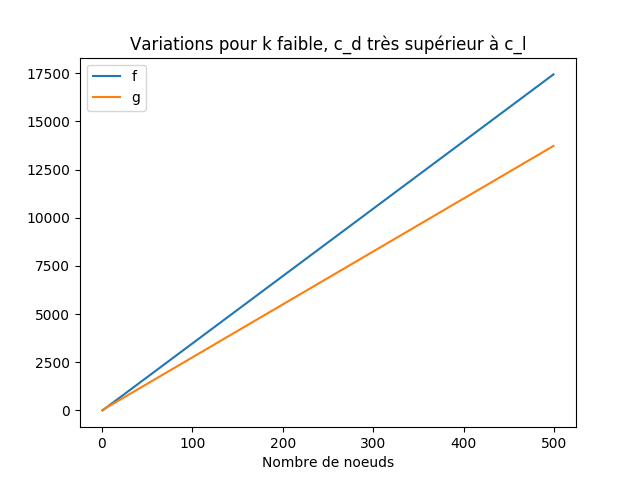
\includegraphics[width=0.49\linewidth]{C:/Users/Dimitri/Desktop/comp5.png}
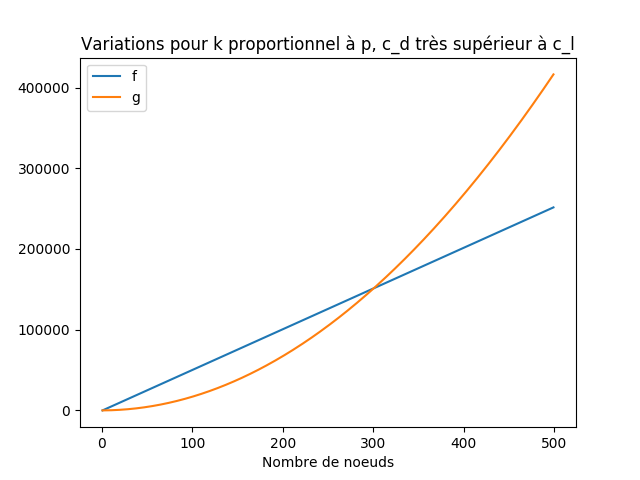
\includegraphics[width=0.49\linewidth]{C:/Users/Dimitri/Desktop/comp8.png}
\captionof{figure}{Variations de f et g en fonction de p.} 
\end{center}

On remarque donc que si la protection d'une arête est chère comparée au coût de sa formation et que la puissance des attaques reste limitée, alors l'organisation d'un réseau selon un graphe de Harary est   avantageuse. Cependant, si l'ampleur des attaques augment avec p, le coût du graphe en étoile devient rapidement plus faible.



\subsection{Analyse - Exploitation - Discussion}
Ces résultats peuvent s'expliquer de la manière suivante : si $k$ varie proportionnellement à $p$, le graphe de Harary doit rester (k+1)-arête connexe pour être suffisamment robuste. Le nombre d'arête de ce graphe, qui est $\lceil (p(k+1)/2) \rceil$, augmente donc de manière équivalente à  p². Un graphe dont les arêtes ne sont pas protégées doit donc avoir un très grand nombre d'arêtes pour rester (k+1)-connexe, ce qui compense la différence de coût, même si elle est élevée, entre une arête protégée et non protégée. Donc pour un grand réseau qui subit des attaques à grande échelle, une organisaton de réseau en étoile est plus optimale.

Le modèle utilisé est limité par deux points qui réduisent sa pertinence en pratique :
	-J'ai considéré que la défense était parfaite, c'est à dire que si un élément était protégé, alors il était impossible de le retirer.
	-Les topologies de ces réseaux sont « utopiques » : un réseau en étoile serait difficile à mettre en place physiquement, par exemple pour un réseau routier. Un modèle plus réaliste serait peut-être plusieurs réseaux en étoile reliés entre eux.
	
\section{Conclusion générale}
Pour conclure, si un réseau n'a à résister qu'à de faibles attaques et que les protections sont coûteuses,  le meilleur réseau est un graphe de Harary. Sinon, il est préférable de construire un réseau où les nœuds sont reliés à un nœud central protégé, avec des liens protégés également. Mon binôme a montré que concevoir des réseaux informatiques invariants d'échelle plutôt qu'homogènes permettait de limiter la propagation d'information fausses en leur sein.




\end{document}
